% !TEX root = mythesis.tex
% !TeX spellcheck = en_GB
%==============================================================================
\chapter{Initial Status of the Picoamperemeters}
\label{sec:current_status}
%==============================================================================
The \ac{pAM} currently in use were designed and built at the TU München. The design was revised multiple times both revision three and four\footnote{Revision 4 was developed by \cite{bugl}.} are in use. The main focus in the following chapters is on the revision three devices, as revision four does not deviate significantly.
The schematics and PCB layout for the design can be found in appendix \ref{sec:rev3}. Before conducting an analysis of the devices and the affiliated infrastructure an introduction on the overall setup is necessary, and therefore provided here.
\section{The Backend Setup}
The control unit of the \ac{pAM} is the \ac{msp} \ac{uC}, which is a low power device produced by \ac{TI}\footnote{For details refer to the manual \cite{msp_manual}.}. It is highly flexible and offers pins with internal compatibility for common protocols as \ac{iic} and \ac{spi}. The \ac{msp} comes with 6 Ports, 8 \ac{IO} pins each, ports 1 and 2 have full interrupt capability. For programming of the MSP430 a JTAG interface is implemented. The firmware running on the MSP coordinating the measurements is described in section \ref{sec:firmwareold}.
The \ac{uC} is driven by a single \SI{3.3}{\volt} supply, fixing the logic levels accordingly.

For communication with an external computer while in operation the devices are equipped with an \acs{xbee} wireless module; which is operated via the USART in- and output ports of the \ac{uC}. The operation of the \acs{xbee} modules is described in \ref{sec:theory:XBee}.

\subsection{Mode Control}
The \ac{pAM} come with multiple modes of sensitivity, depending on the revision. Mode switching and the turn on/off are combined in one circuit as depicted in figure \ref{fig:backend:modeswitching:circuit}. Cycling the modes is handled in the Reed interrupt routine, according to figure \ref{fig:backend:modeswitching}. %This is handled in the %\code{port1_isr(void)}
\begin{figure}
	\begin{subfigure}{0.49\textwidth}
		\centering
		\includegraphics[width=\textwidth]{../../../Figures/backend/switching/switching_circuit.pdf}
		\caption{Mode switching and reed interrupt trigger for the \ac{pAM} revisions 3 and 4.}
		\label{fig:backend:modeswitching:circuit}
	\end{subfigure}\hfill
	\begin{subfigure}{0.49\textwidth}
		\centering
		\includegraphics[width=0.8\textwidth]{../../../Figures/backend/switching/switching.png}
		\caption{Reed interrupt cycling through the different modes and turning on and off of the device. From \cite{roedel}.}
		\label{fig:backend:modeswitching}
	\end{subfigure}
\caption{Implementation of mode switching in the \ac{pAM} revision 3 and 4.}
\end{figure}

\section{The Front-end Setup}
The \ac{pAM} measure current indirectly by determining the voltage drop over a shunt resistor, following Ohm's law. This is done by the use of an \ac{opamp}\ in a simple amplifier configuration, as depicted in figure \ref{fig:shuntamp}.
\begin{figure}
	\centering
	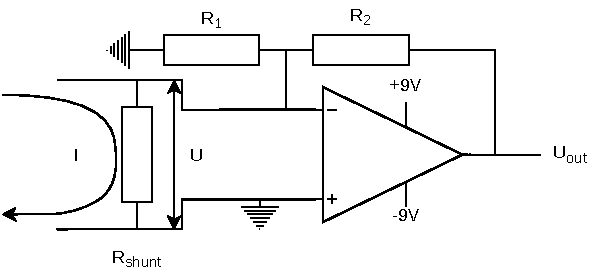
\includegraphics[width=.4\textwidth]{../../../Figures/shuntamp_sketch/shuntamp.pdf}
	\caption{Current measurement circuit using an operational amplifier and a shunt resistor.}
	\label{fig:shuntamp}
\end{figure}
Using Ohm's law and the golden rules of operational amplifiers, see section \ref{sec:theory:amplifiers}, the simple relation in equation \ref{eq:shuntamp} can be derived.
\begin{align}
	U_\text{out} & = R_\text{S}I\label{eq:shuntamp}
\end{align}
This first amplification stage uses an AD549LHZ \ac{opamp} which features a high input impedance, low input current and offset voltage adjustment \cite{AD549}. According to its datasheet, it is designed to be used for electrometer amplifiers or photodiode interfaces. Driving the amplifier with a bipolar supply allows measurement of both positive and negative currents. For matching the bipolar voltage signal from the input stage with the unipolar \ac{adc} input, a second amplifier is introduced as depicted in figure \ref{fig:frontendsketch}, expanding equation \ref{eq:shuntamp} to:
\begin{align}
	U_\text{ADC}=IR_\text{S}+U_\text{ref}
	\label{eq:frontend:old:transferfunction1}
\end{align}
Where $U_\text{ref}=\SI{2.048}{\volt}$.
\begin{figure}
	\centering
	\includegraphics[width=.8\textwidth]{../../../Figures/shuntamp_sketch/frontendsketch.pdf}
	\caption{Front-end circuitry used in the revisions 3 and 4. The additional \ac{ovp} diodes are depicted in figure \ref{fig:frontend:old:ovp2}.}
	\label{fig:frontendsketch}
\end{figure}
As a second amplifier, the $\mu$A741 is used. It is a general-purpose amplifier, designed for voltage amplification.
For digitisation, the design uses the AD7790 buffered $\Sigma\Delta$ \ac{adc} which features a suitable low noise for the application and has a sampling frequency of \SI{9.5}{} to \SI{120}{\hertz} \cite{AD7790}. Taking into account the digitisation range of the \ac{adc} and the highest shunt resistance of \SI{100}{\mega\ohm} the setup could reach a theoretical precision of \SI{0.625}{\pico\ampere}. 

\subsection*{Over-Voltage Protection}
\label{sec:status:ovp}
The \acp{pAM} are equipped with protection diodes as depicted in figure \ref{fig:frontend:old:ovp1}, to prevent damage to the amplifier from over-voltage conditions. In figure \ref{fig:frontend:old:ovp2} an extension to the input stage is depicted, which is soldered floating over the board. It consists of a \SI{20}{\kilo\ohm} resistor in parallel to a SA5.0CA bipolar TVS diode\footnote{It is unknown why this circuitry was attached or by whom. It was already mentioned in \cite{bugl} in 2013.}. The resistor forms a voltage divider with the \SI{5}{\kilo\ohm} resistor, adding an extra factor to the transfer function. The transfer-function in equation \ref{eq:frontend:old:transferfunction1} is expanded to:
\begin{align}
U_\text{ADC}=1.25\cdot IR_\text{S}+U_\text{ref}
\label{eq:frontend:old:transferfunction2}
\end{align}
The influence of the TVS diode will be discussed in section \ref{sec:nonlinearity}.
\begin{figure}
	\begin{subfigure}{\textwidth}
		\centering
		\includegraphics[width=0.8\textwidth]{../../../Figures/shuntamp_sketch/frontendsketchwOVP1.pdf}
		\caption{Front-end equipped with over voltage protection diodes between the inputs of the first amplifier.}
		\label{fig:frontend:old:ovp1}
	\end{subfigure}\hfill
	\begin{subfigure}{\textwidth}
		\centering
		\includegraphics[width=0.8\textwidth]{../../../Figures/shuntamp_sketch/frontendsketchwOVP2.pdf}
		\caption{The same front-end with additional \SI{20}{\kilo\ohm} resistor and parallel SA5.0CA TVS-diode.}
		\label{fig:frontend:old:ovp2}
	\end{subfigure}
	\caption{The two expansions that are made to the front-end depicted in figure \ref{fig:frontendsketch}.}
\end{figure}
\subsection*{Selectable Modes}
As introduced before the \acp{pAM} have a selectable resolution and measurement range. This is achieved by adding a second smaller resistor $R_\text{||}$ in parallel to the \SI{100}{\mega\ohm} resistor; this reduces the shunt resistance to:
\begin{align}
	R_\text{S}=\frac{1}{\frac{1}{R_{||}}+\frac{1}{\SI{100}{\mega\ohm}}}
\end{align} 
Modes for the different revisions are shown in table \ref{tab:frontend:old:modes}. The low-resolution modes also use a varistor parallel to the shunt resistor as additional over-voltage protection.
\begin{table}
	\centering
	\begin{tabular}{cccccc}
		\hline
		mode & shunt resistance & range & resolution & \multicolumn{2}{c}{raw mode} \\
		 & 						 & & 		& revision 3 & revision 4 \\
		\hline
		1 & \SI{100}{\ohm}$||$\SI{100}{\mega\ohm} & \SI{\pm16.4}{\milli\ampere} & \SI{625}{\nano\ampere} & 0 & \\
		2 & \SI{10}{\kilo\ohm}$||$\SI{100}{\mega\ohm} & \SI{\pm164}{\micro\ampere} & \SI{6.25}{\nano\ampere} & 1 & 0 \\
		3 & \SI{100}{\kilo\ohm}$||$\SI{100}{\mega\ohm} & \SI{\pm16.4}{\micro\ampere} & \SI{625}{\pico\ampere} & & 1 \\
		4 & \SI{1}{\mega\ohm}$||$\SI{100}{\mega\ohm} & \SI{\pm1.64}{\micro\ampere} & \SI{6.25}{\pico\ampere} & 2 & 2 \\
		5 & \SI{10}{\mega\ohm}$||$\SI{100}{\mega\ohm} & \SI{\pm164}{\nano\ampere} & \SI{0.625}{\pico\ampere} & & 3 \\
		6 & \SI{100}{\mega\ohm} & \SI{\pm16.4}{\nano\ampere} & \SI{0.5}{\pico\ampere} & 3 & 4 \\
		\hline
	\end{tabular}
	\captionof{table}{Modes of the different \ac{pAM}, the range is given by $\frac{\text{\SI{2.048}{\volt}}}{1.25\text{R}_\text{S}}$. This sets the resolution to range divided by $2^{15}$. Translated and modified from \cite{rudolph}.}
	\label{tab:frontend:old:modes}
\end{table}
\section{High-Voltage Isolation}
The \acp{pAM} are designed for usage on the high-voltage supply lines of a \ac{gem}-foil. This requires some precautions to protect a user. To ensure isolation, the \acp{pAM} are enclosed in a plastic box. The only openings in this box are the terminals for the signal lines. The terminals are SHV connectors, the outer conductor is connected to earth ground, only the inner conductor is on a high-voltage. \\
As a power supply the devices use \SI{9}{\volt}-blocks, as these allow operation without any ground connection. In addition, a photovoltaic powering was developed, to achieve longer run times, see \cite{rudolph} for details.
\section{Design Performance}
\subsection{Power Consumption}
The power consumption characteristics were studied by \cite{rudolph} and are only briefly summarized here. Originally the devices are powered by \SI{9}{\volt}-block batteries, hence low power consumption is a design goal. Table \ref{tab:frontend:old:power} summarizes the current draw for an operating device.
\begin{table}
	\centering
	\begin{tabular}{lr}
		\hline
		Average & current draw \SI[per-mode=symbol]{}{\per\milli\amp}\\ \hline
		without XBee & \SI{1.773\pm0.012}{} \\
		with the Xbee sending & \SI{48.1\pm0.6}{} \\
		\hline
	\end{tabular}
	\captionof{table}{Current draw of a \ac{pAM}. From \cite{rudolph}, modified.}
	\label{tab:frontend:old:power}
\end{table}
\subsection{Measurement Results}
The measurement performance of the device was analysed by \cite{roedel}. It was found that the devices show a characteristic non-linear behaviour with deviations in the range of some ten \ac{pA} in the most sensitive mode. This non-linearity scales linear with temperature, which was also shown by \cite{roedel}. The origin of the effect is discussed in section \ref{sec:nonlinearity}.

Calibration measurements showed that the error on the \ac{pAM} reading, the standard deviation of 128 measurements, is around 1.5 to 2 \ac{adc} channels, resulting in an uncertainty of around \SI{1}{\pico\amp}. Showing that the design is capable of precise measurements on the \ac{pA} scale.

The \ac{pAM} take \SI{8}{\second} to finish a complete sample of 128 \ac{adc} readings. This is mainly due to the low \ac{adc} sampling rate that is used. This low sample rate results in a bad time resolution.

\section{Infrastructure}
To operate the \ac{pAM} the firmware for the \ac{uC} is needed, as well as the \ac{pamos} software; which is responsible for receiving the data, applying the calibration and saving the results. To obtain a reliable calibration for the \acp{pAM}, a calibration station was built by \cite{roedel}. A short introduction to the software is given here.
\subsection{Firmware}
\label{sec:firmwareold}
With the beginning of this thesis, the \ac{msp} firmware is present in versions 3 and 4 for the respective revisions of the design. It is written in C and compiled via the opensource msp430-gcc compiler in version 3.2.3; which is only running on Ubuntu 10.04.4 LTS, according to \cite{agwiki}. The rather complicated flashing process is described there as well. 
The basic workflow of the firmware is depicted in figure \ref{fig:firmware:old:workflow}.\\
\begin{figure}
	\centering
	\includegraphics[width=.8\textwidth]{../../../Figures/pAMworkflow/old/mainloop/main.pdf}
	\caption{\ac{pAM} firmware workflow for firmware versions 3.x.}
	\label{fig:firmware:old:workflow}
\end{figure}
The firmware comes in different builds featuring different functionalities. The firmware versions x.0 are the basic versions, the versions x.1 additionally send out all 128 \ac{adc} raw values. All firmware versions also have a second build, that sets the \textit{CALIB} flag, which adds auto mode switching to the firmware.

To simplify coding and increase readability of the code, a lot of alternative symbols are defined in the header files \textit{iostructures.h} and \textit{pAM-definitions.h}. 
The ports and pins were assigned an alias according to their purpose. For example, the \ac{adc} communication is done with port 3, pins 0 to 3, hence the aliases are:
\begin{lstlisting}[style=cpp]
#define ADC_PORT port3
#define ADC_SCLK pin3 /* P3.3 SCLK */
#define ADC_DOUT pin2 /* P3.2 SOMI */
#define ADC_DIN pin1 /* P3.1 SIMO */
#define ADC_CNV pin0 /* P3.0 */
\end{lstlisting}


\subsubsection*{Initilisation}
On start-up of the microcontroller, some basic settings have to be made. At first, the clock and timer modules have to be set up. The device is equipped with a \SI{32}{\kilo\hertz} crystal on \pin{XIN} and a \SI{1.8}{\mega\hertz} crystal on \pin{XT2}. As main clock source in the \acp{pAM}, the \SI{1.8}{\mega\hertz} clock is used.

The next step is to set up the pins according to their purpose. Each port has several registers defining their usage, see table \ref{tab:firmware:portregisters}. This happens with the function \code{port\_setup()}, the registers for the different ports are summarized in table \ref{tab:firmware:portregisters}.
\begin{table}
	\centering
	\begin{tabular}{clccccc}
		\hline
		register & register purpose &\multicolumn{3}{c}{ports}&\multicolumn{2}{c}{states} \\
		 & & 1 & 2 & 3 - 6 & 1 & 0 \\\hline 
		dir & select if pin is input or output &\checkmark&\checkmark&\checkmark& output & input \\
		in & state applied to pin &\checkmark&\checkmark&\checkmark& \multicolumn{2}{c}{set externally}\\
		out & state applied to pin &\checkmark&\checkmark&\checkmark& set output high & set output low \\
		sel & function selection &\checkmark&\checkmark&\checkmark& peripheral module & I/O functionality\\
		ie & interrupt enable &\checkmark&\checkmark& & interrupt enabled & interrupt disabled\\
		ies & interrupt edge select &\checkmark&\checkmark&& falling edge & rising edge\\
		ifg & interrupt flag &\checkmark&\checkmark&& interrupt pending & no interrupt pending \\
		\hline
	\end{tabular}
	\captionof{table}{Registers, their purpose and ports that feature them. Only ports 1 and 2 have interrupt capability \cite{msp_manual}.}
	\label{tab:firmware:portregisters}
\end{table}
The USART module is set up to interface the \acs{xbee}, as depicted in listing \ref{lst:firmware:old:usart}. The modules setup allows two-way communication. However, the communication protocols for this are not implemented.
\begin{codecpp}[caption={Setup of the USART ports for communication with the \acs{xbee} \label{lst:firmware:old:usart}. Comments preceded with \textit{//<} were added for explanation.}]
void usart_setup() {
	/*TX*/
	//<TX pin for transmitting data: 
	port3.dir.pin4 = IO_DIRPIN_OUTPUT; //<=1
	port3.sel.pin4 = IO_ALTPIN_SELECT;//<=1
	/*RX*/
	//<RX pin for receiving data:
	port3.dir.pin5 = IO_DIRPIN_INPUT; //<=0
	port3.sel.pin5 = IO_ALTPIN_SELECT;//<=1
	
	ME1 |= UTXE0 + URXE0; // USART0 TX, RX enable
	//<set protocol to 8 data-bits, 1 stop-bit, no parity (8N1):
	U0CTL |= CHAR;		 // 8 data-bits, 1 stop-bit, no parity (8N1)
	//< set clock source to MCLK (1.8MHz): 
	U0TCTL |= SSEL_2;	 // UCLK <- SMCLK	
	/* clock: 1843200Hz
	desired baud rate: 115200bps
	division factor: 16
	effective baud rate: 115200bps
	maximum error: 0us 0.00%
	*/	
	//< set divider to 16, 	modulation to 0:
	U0BR0=0x10; U0BR1=0x00;	U0MCTL=0x00;
	//<open USART for operation:
	U0CTL &= ~SWRST;			/*USART freigeben*/
}
\end{codecpp}
After these setups, the mainloop is started. First the \ac{adc} is reset, and the LED blinks to signal operation. After this the \ac{adc} is setup for reading data. The firmware reads 128 values from the \ac{adc}, entering a low power mode in between conversions. The \ac{adc} \pin{RDY} pin is used as an interrupt to enter the corresponding \ac{ISR}, which handles data reading.

After data is read-out, mean and standard deviation of the 128 values is calculated. This averaging has the advantage of reducing the influence of noise on the data and allows more precise measurements. However, it elongates the readout time. The derived values get sent out along with other parameters. The data frame for the firmware revisions x.0 is depicted in figure \ref{fig:firmware:vx0:dataframe}; the versions x.1 packages are shown in figure \ref{fig:firmware:vx1:dataframe}. Afterwards, the readout is finished, and another cycle starts.
\begin{figure}
	\centering
	\begin{tabular}{|C{4cm}|C{4cm}|C{1cm}|C{1cm}|C{1cm}}
		\cline{1-4}
		mean & error & mode & voltage & \dots \\
		\cline{1-4}
		\multicolumn{5}{c}{}
		%\mc{4 byte} & \mc{4 byte} & \mc{1 byte} & \mc{1 byte} \\ 
	\end{tabular}
	\begin{tabular}{C{1cm}|C{4cm}|C{4cm}|C{1cm}|}
		\cline{2-4}
		\dots & conversion time & time until sending & 0\\
		\cline{2-4}
		\multicolumn{4}{c}{}
		%\multicolumn{}{c}{}
		%\mc{4 byte} & \mc{4 byte} & \mc{1 byte} & \mc{1 byte} \\ 
	\end{tabular}
	\captionof{figure}{Datasets as sent out by \acp{pAM} running the firmware v3.0 and v4.0. The package contains mean and error of the acquired data, the current operating mode, the SVS voltage output, the time needed for conversion, the time between finishing a conversion and sending data, and the number of remaining packages; which is 0 in this case.}
	\label{fig:firmware:vx0:dataframe}
\end{figure} 
\begin{figure}
	\centering
	\begin{tabular}{|C{4cm}|C{4cm}|C{1cm}|C{1cm}|C{1cm}}
		\cline{1-4}
		mean & error & mode & voltage & \dots \\
		\cline{1-4}
		\multicolumn{5}{c}{}
		%\mc{4 byte} & \mc{4 byte} & \mc{1 byte} & \mc{1 byte} \\ 
	\end{tabular}
	\begin{tabular}{C{1cm}|C{4cm}|C{4cm}|C{1cm}|}
	\cline{2-4}
	\dots & conversion time & time until sending & 4\\
	\cline{2-4}
	\multicolumn{4}{c}{}
	%\multicolumn{}{c}{}
	%\mc{4 byte} & \mc{4 byte} & \mc{1 byte} & \mc{1 byte} \\ 
	\end{tabular}
	\begin{tabular}{|C{2cm}|C{2cm}|C{3cm}|C{2cm}|C{1cm}|}
	\cline{1-5}	%\cline{4-5}
	\ac{adc} value & \ac{adc} value & \dots &\ac{adc} value & 3\\
	\cline{1-5}	%\cline{4-5}
	\ac{adc} value & \ac{adc} value & \dots &\ac{adc} value & 2\\
	\cline{1-5}	%\cline{4-5}
	\ac{adc} value & \ac{adc} value & \dots &\ac{adc} value & 1\\
	\cline{1-5}	%\cline{4-5}
	\ac{adc} value & \ac{adc} value & \dots &\ac{adc} value & 0\\
	\cline{1-5}	%\cline{4-5}
	%\mc{4 byte} & \mc{4 byte} & \mc{1 byte} & \mc{1 byte} \\ 
	\end{tabular}
	\captionof{figure}{Datasets as sent out by \ac{pAM} running the firmware v3.1 and v4.1. The first package contains mean and error of the acquired data, the current operating mode, the SVS voltage output, the time needed for conversion, the time between finishing a conversion and sending data, and the number remaining packages. The next four packages contain 32 \ac{adc} readings each, followed by the number of remaining packages.}
	\label{fig:firmware:vx1:dataframe}
\end{figure} 

\subsection{\acs{pamos}}
The \acl{pamos} is the software used to receive and handle data, send out by the \acp{pAM}. It is written in \acs{cpp} to be run on Linux machines. With the beginning of this work, it was available in version 2. The software reads data, applies the calibration and stores data in an online database or locally as a root file. Discrimination between the firmware versions described above is done by the message length. 

\subsection{CalibAna}
The CalibAna software was developed by \cite{roedel}. A detailed description of its principle can be found there. It controls the calibration setup by communicating with, an Arduino to adjust the temperature, the \ac{keithley}, which used as a reference for calibration and reads the \ac{pAM} data. The output can be stored in a calibration database and be used to create a plot with the calibration data, using a gnuplot script. An example plot is shown on figure \ref{fig:CalibAna2:example}. The top left plot shows current measured by the Keithley vs \ac{adc} readings and a linear fit of the data. The central plot contains the deviation of current values from the linear fit applied to the \ac{adc} channel range. These deviations are fitted with a third-order polynomial. The bottom left plot shows the deviations from the polynomial fit as a histogram. A gaussian fitted to the histogram is used to approximate the resolution of the \ac{pAM}. 
\begin{figure}
	\centering
	\includegraphics[width=\textwidth]{../../../Figures/pAMOld/Measurements/cal_stat16_rmode0_rand_temp_2017-01-18_00.34_plot.pdf}
	\caption{Calibration plot produced by CalibAna2.}
	\label{fig:CalibAna2:example}
\end{figure}


\section{Motivation}
Now, having provided a look into the device, why is a revision of the design necessary?
There are several shortcomings in operation and handling of the design that were discovered over time. 
As described above, the firmware is not up to date and is not compatible with modern compilers. Hence upgrading the firmware is one of the bullet points.
This process can also be used to add new features to the firmware to make operation of the device more flexible.

A problem that occurs during operation is a breakdown of the \ac{opamp} in the input stage, probably due to over-voltage conditions on the inputs. On the one hand, replacement of an amplifier is complex and rather costly with $\approx$\SI{60}{\euro} per amplifier.  On the other hand, the running measurement is interrupted and needs to be repeated. \\
One of the biggest issues, in the end, is non-linear current to \ac{adc} channels relation mentioned above in combination with a temperature dependence, making a complex and time-consuming calibration necessary.
%It was desired to have the ability to see the measurement result in real time over a display, this was addressed by \cite{bugl}, but lead to a more noisy measurement in operation.








